% 第 18 题圆 M 坐标图：按固定源 PDF 矢量路径换算（1 pt → 0.03515 cm）。
% 原点取 O（源页 (1030.25, 675.27) pt），y 向上。
% 圆线宽 0.8pt（其余图元 2 倍）；圆心 M (55.43,64.66)、半径 46.19；
% 圆上定点 A（题设 A(2,4) 的精确作图位置，正比 9.238 pt/单位）；M、A 处实心点。
% x 轴左 −18.48 右至箭头尖点 110.85；y 轴下 −18.48 上至箭头尖点 120.09。
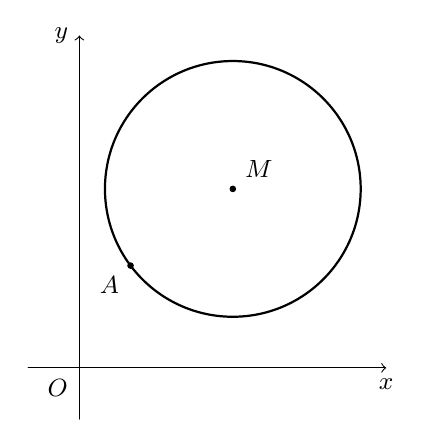
\begin{tikzpicture}[line cap=round,line join=round,font=\small,x=0.03515cm,y=0.03515cm]
% 坐标轴
\draw[->] (-18.48,0)--(110.85,0);
\draw[->] (0,-18.48)--(0,120.09);
% 圆（线宽 0.8，与源一致）
\draw[line width=0.8pt] (55.43,64.66) circle (46.19);
% 实心点（M、A）
\fill (55.43,64.66) circle (1.2pt);
\fill (18.48,36.95) circle (1.2pt);
% ===== 标注（照源字框中心，显式坐标）=====
\node[anchor=center,inner sep=0] at (-6.50,120.09) {\(y\)};
\node[anchor=center,inner sep=0] at (64.83,71.94) {\(M\)};
\node[anchor=center,inner sep=0] at (10.88,29.84) {\(A\)};
\node[anchor=center,inner sep=0] at (-7.85,-7.29) {\(O\)};
\node[anchor=center,inner sep=0] at (110.77,-5.96) {\(x\)};
\end{tikzpicture}
